%\chapter{Construcción de supercondensadores}
Un supercondensador es construido haciendo el sándwich electrodo-separador-electrodo más la adición de un electrolito. Éste último, es una solución acuosa de hidróxido de potasio (\ce{KOH}) a una concentración 6M, la que es utilizada ampliamente en este tipo de estudios \citep{Frackowiak2001}.  El material que servirá de electrodo debe estar depositado en un colector de corriente, o ser una lámina libre, en este trabajo los electrodos los conforman láminas de grafeno, mientras que los colectores son discos de acero inoxidable UNS316L, que presenta mayor resistencia a la corrosión por hidróxido de potasio. Por otro lado, el separador es una membrana permeable al electrolito, el cual puede ser una membrana microporosa o papel filtro de celulosa, este último es el empleado en esta tesis.

La primera aproximación a la construcción del supercondensador se explica en la secuencia de la figura \ref{fig:SC_process}. Primero se adhiere el colector de corriente metálico a un sustrato de vidrio. Segundo, se delimita el área a depositar mediante una cinta adhesiva. Tercero se deposita mediante goteo la solución de grafeno en el colector de corriente. Cuarto, se evapora el líquido dispersante . Quinto, se añaden gotas de electrolito. Sexto, se cierra el sistema con un segundo electrodo.

\begin{figure}[h!]
	\centering
	\fbox{
		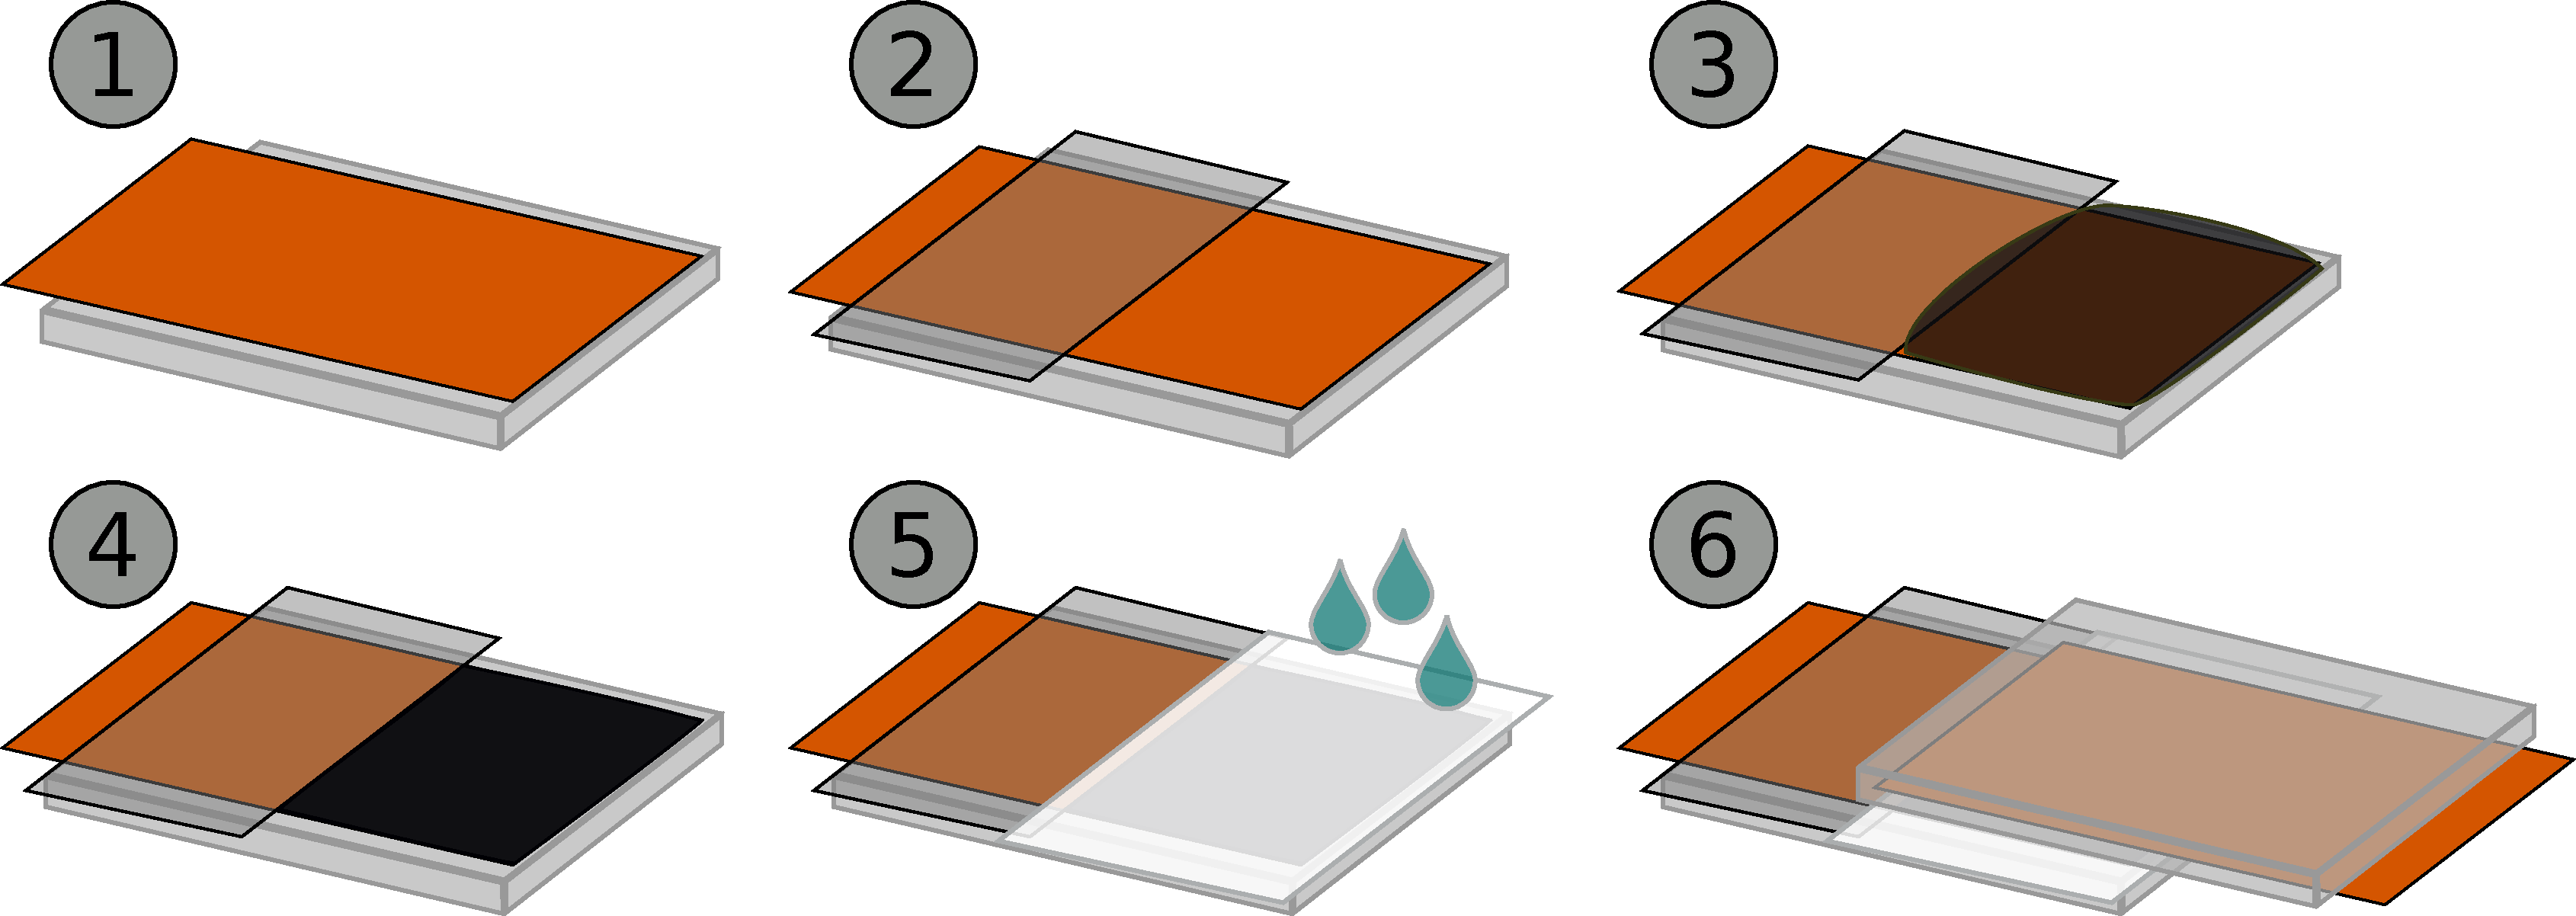
\includegraphics[width = 0.9\textwidth]{SC_process.pdf}
		}
	\caption[Principio de contrucción de un supercondensador]{Secuencia para la construcción de un supercondensador básico.}
	\label{fig:SC_process}
\end{figure}

\section{Celda de pruebas de supercondensador}
La construcción de supercondensadores como se detalla anteriormente, presenta varios inconvenientes: (1) los colectores de corriente de aluminio y cobre utilizados, se degradan rápidamente al exponerse al electrolito (KOH). (2) la deposición de material en los colectores de corriente no es homogénea, generando zonas donde el colector queda expuesto al electrolito. (3) el agua del electrolito se evapora rápidamente, disminuyendo la cantidad de iones en el medio de conducción. (4) el cierre del dispositivo no es estable y no permite su reproducibilidad, y por consiguiente (5) la conexión a los terminales eléctricos no es estable. Por estas razones y conservando los principios básicos de la construicción de supercondensadores, se diseña una celda de pruebas para solucionar estos problemas.

La celda diseñada y construida (figura \ref{fig:celda_de_pruebas_SC}), consta de dos colectores de corriente de acero inoxidable, entre los que se ubica el supercondensador. Los colectores de corriente tienen juntas tóricas que impiden la fuga del electrolito o la evaporación del agua en él, permitiendo una operación estable en el tiempo. Los colectores de corriente se apoyan en bloques de acero que aseguran la celda con cuatro pernos, permitiendo conectar los terminales del potenciostato a la celda de pruebas.

\begin{figure}[h!]
	\centering
	\fbox{
		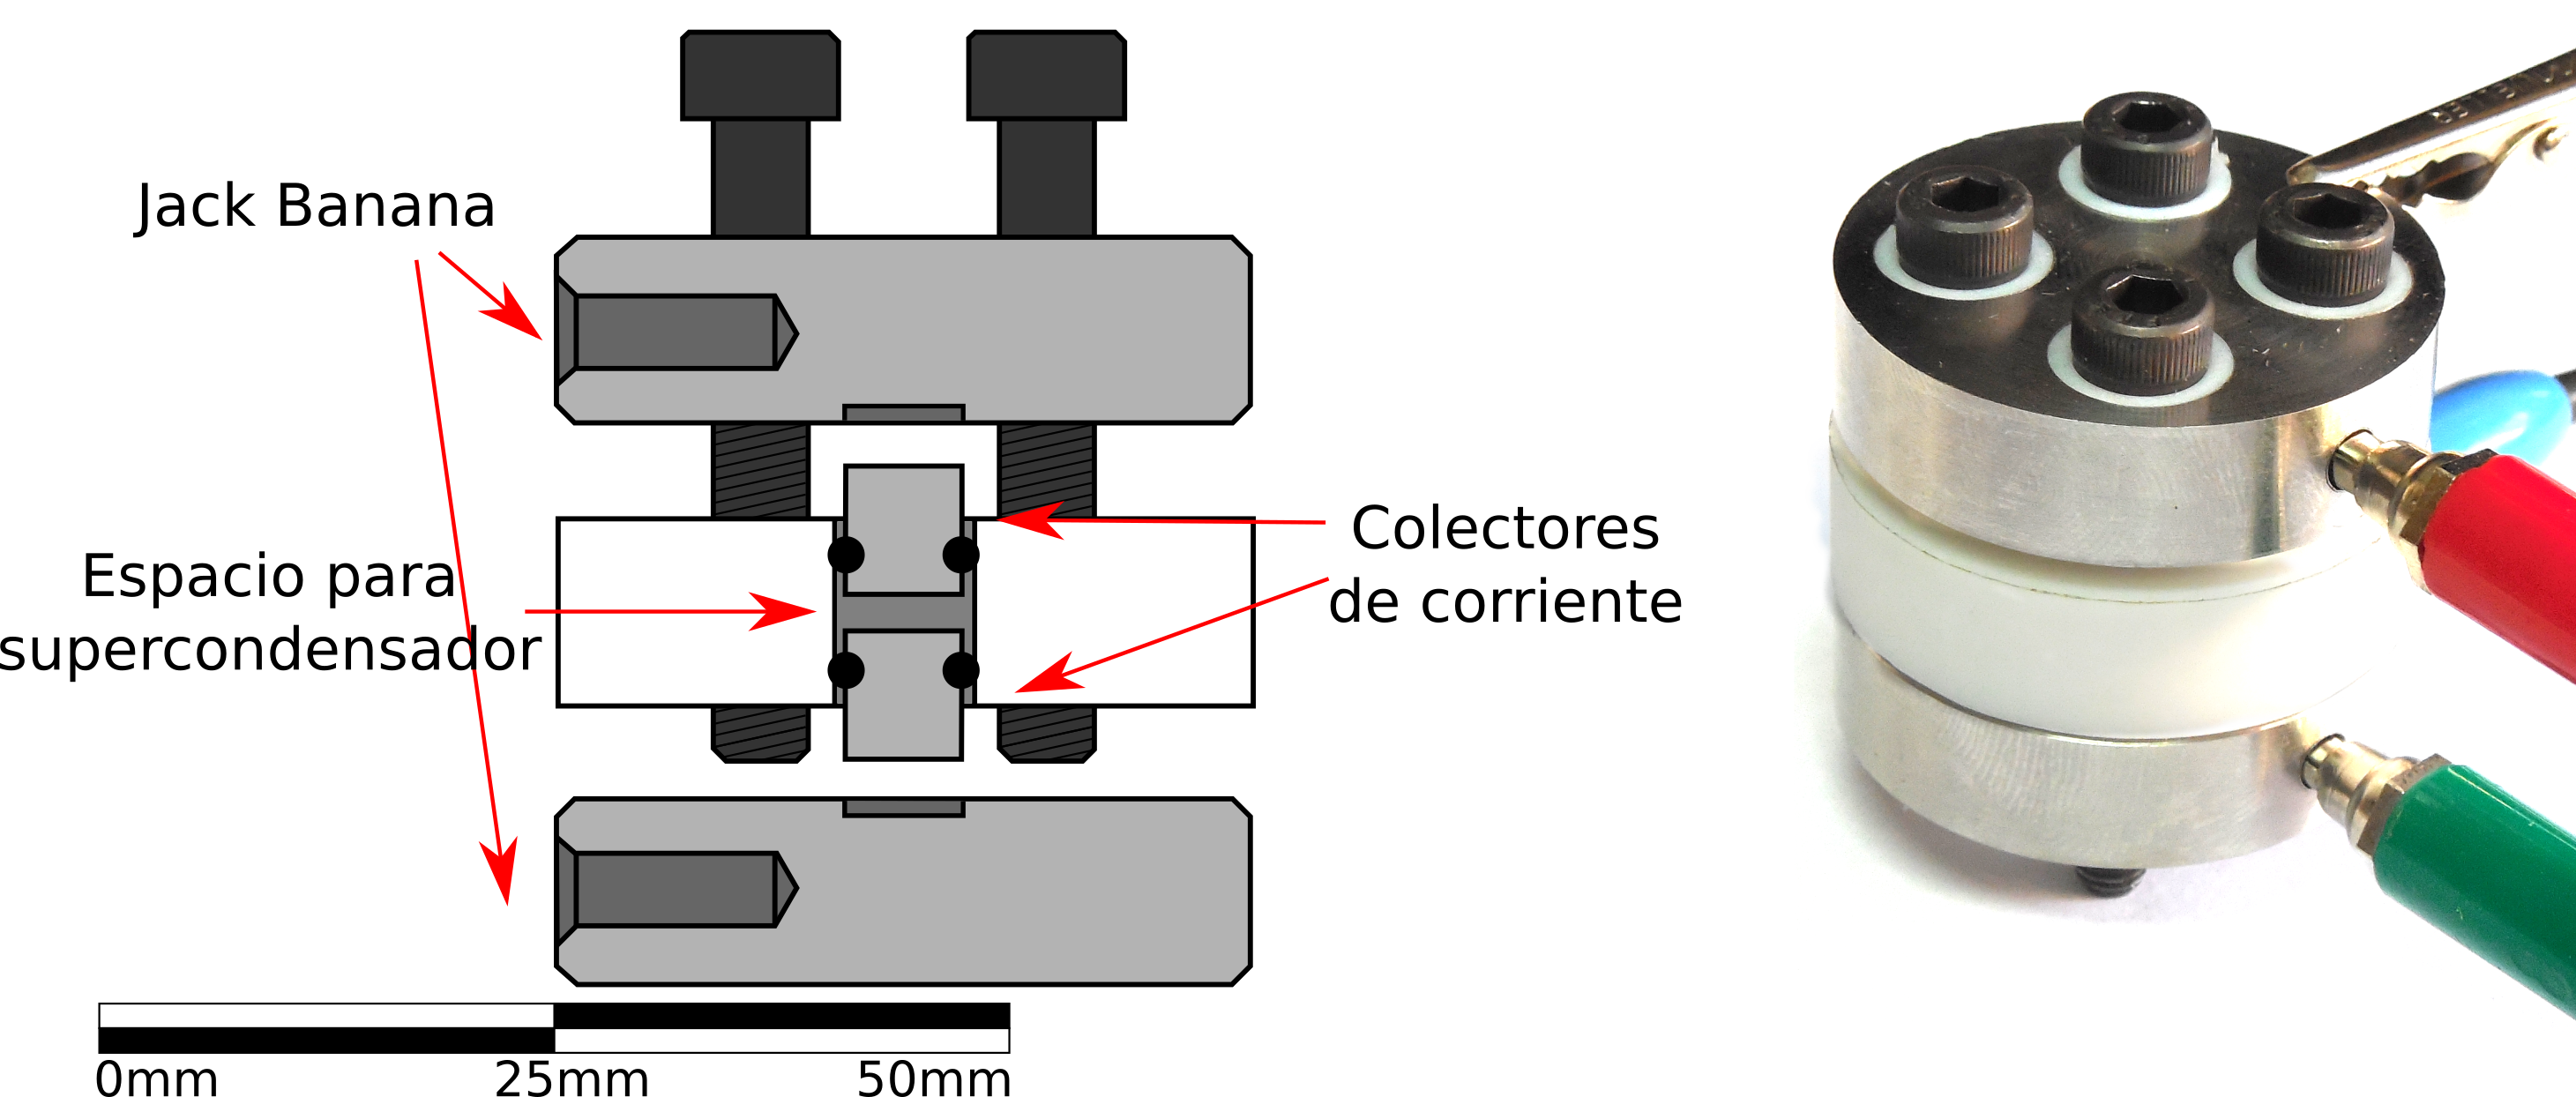
\includegraphics[width=0.8\textwidth]{cell3.pdf}
		}
	\caption[Celda de pruebas de supercondensador]{Izquierda: Vista en corte longitudinal de la celda de pruebas mostrando los componentes más importantes. Derecha: Fotografía de la celda armada y conectada al potenciostato.}
	\label{fig:celda_de_pruebas_SC}
\end{figure}

\section{Construcción de electrodos}
Se fabrican seis pares de electrodos utilizando el mismo material sintetizado, pero diferentes sustratos y diferentes métodos de deposisión. Se utilizan dos tipos de sustratos, el primero es un disco de acero de 7 mm de díametro, el segundo es un disco de espuma de níquel también de 7 mm de diámetro, que tiene mayor área superficial (EQ-bcnf-16m, MTI Corporation). Para fabricar el primer par de electrodos, el material en forma de polvo es dispersado ultrasonicamente en etilenglicol, que mostró mayor homogeneidad que el agua para la deposición de rGO, y depositado por goteo hasta cubrir completamente el sustrato de acero previamente calentado a 150 \degree C. Un segundo par se fabrica añadiendo polimetilmetacrilato (PMMA), a la solución a depositar, este se disuelve en acetona a una concentración de 10 mg/ml, solución donde se dispersa el óxido reducido de grafeno por medio de ultrasonido y luego es depositada por goteo en el sustrato de acero a 50 \degree C. De forma análoga, el tercer y cuarto par repiten los procesos anteriores pero cambiando el sustrato de acero por el de níquel. Manteniendo el sustrato de acero, el quinto par consiste en electrodos de papel fabricados mediante filtración por vacío. En este método, se dispersa el rGO en agua, la que se pasa por un filtro de celulosa en un embudo Büchner conectado a un kitasato y una bomba de vacío, el filtro con el material atrapado se deja secar a temperatura ambiente formando una lámina, la que es desprendida con facilidad del filtro y luego recortada al tamaño apropiado para la celda de pruebas (7 mm). El material dispersado en agua también puede ser liofilizado, obteniendo una espuma de rGO que es utilizada como electrodo en la celda.
%TODO balanza
La masa del material depositado se mide en una balanza analítica (), conociendo previamente la masa de los sustratos y teniendo la precaución que el solvente se haya evaporado totalmente. Para los discos de papel de rGO, se masan 20 de ellos y se calcula la masa promedio de cada uno. En el caso del material liofilizado, se masa directamente la cantidad a utilizar en la celda de pruebas. En la tabla \ref{tab:electrodos_construidos} se resumen los electrodos fabricados, detallando la masa de material activo.

\begin{table}[htbp]
	\centering
	\caption{Muestras}
	\begin{tabular}{ l l l l l c }
		Nombre	&	Sustrato & Formato       & Aglutinate & Masa [mg]     & Caracterización electroquímica \\
		\hline
		\mSustratoAcero		&	Acero    &   -           & -      &  -            & Figura \ref{SCGraphs:CV_Steel_Disk_No_Material_1} \\
		\mPolvoAcero			&	Acero    & Polvo         & -      & 0,4 $\pm$ 0,2 & Figura \ref{SCGraphs:CV_CRGO300517_9}             \\
		\mPolvoAceroPMMA	&	Acero    & Polvo         & PMMA   & 2,8 $\pm$ 0,2 & Figura \ref{SCGraphs:CV_CRGO300517_3}             \\
		\mPapelAcero		&	Acero    & Papel         & -      & 0,6 $\pm$ 0,1 & Figura \ref{SCGraphs:CV_CRGO300517_11}            \\
		\mLiofilizadoAcero	&	Acero    & Liofilizado   & -      & 0,6 $\pm$ 0,1 & Figura \ref{SCGraphs:CV_CRGO300517_13}            \\
		\mSustratoNiquel	&	Níquel   &  -            & -      &    -          & Figura \ref{SCGraphs:CV_Nickel_Foam_No_Material_1}\\
		\mPolvoNiquel		&	Níquel   & Polvo         & -      & 0,9 $\pm$ 0,2 & Figura \ref{SCGraphs:CV_CRGO300517_5}             \\
		\mPolvoNiquelPMMA	&	Níquel   & Polvo         & PMMA   & 0,8 $\pm$ 0,2 & Figura \ref{SCGraphs:CV_CRGO300517_7}             \\
	\end{tabular}
	\label{tab:electrodos_construidos}
\end{table}

\begin{figure}
	\centering
	\fbox{
		\includegraphics[width=1.0\textwidth]{rgo_electrodes.png}
		}
	\caption[Electrodos utilizados en la celda de pruebas de supercondensador]{Electrodos utilizados en la celda de pruebas de supercondensador. De izquierda a derecha: Electro sin material depositado. Electrodo con material depositado mediante goteo (\emph{drop-casting}). Electrodo con material en forma de papel descentrado. Electrodo con material en forma de papel bien centrado sobre el metal.}
	\label{fig:electrodes}
\end{figure}

\section{Caracterización electroquímica}
Los electrodos son sometidos a pruebas electroquímicas para estudiar su desempeño, estás pruebas incluyen: voltametría cíclica (CV), ciclos de carga y descarga a corriente constante, espectroscopía de impedancia electroquímica (EIS). Todas las mediciones electroquímicas son hechas con un potenciostato/galvanostato Gamry (Interface 5000E). Además de los electrodos construidos con rGO, también se mide el comportamiento de los sustratos de acero y níquel.

La metodología de medición para cada muestra es la siguiente: inicialmente se mide la masa de material depositado. Luego, se limpia la celda de pruebas con etanol, para eliminar cualquier residuo de mediciones anteriores. Posteriormente se arma el supercondensador al interior de la celda, agregando una gota de electrolito al separador de papel y cerrándola con la precaución de que las juntas tóricas sellen correctamente el interior de la celda. Inmediatamente se prosigue con las mediciones electroquímicas. Primero se realizan ciclos de voltametría a diferentes velocidades de barrido: 25, 50, 100, 200, y 400 mV/s, tres ciclos para cada una, y solo se toma la última curva (esto para remover la carga acumulada en el dispositivo bajo prueba).  Luego de la voltametría cíclica, el espectro de impedancia es obtenido y se procede con los ciclos de carga y descarga a corriente constante a 1 A/g, exceptuando las muestras de polvo más pmma en disco de acero y polvo en espuma de níquel, donde la densidad de corriente se disminuyó 0,1 A/g debido a la alta resistencia en serie equivalente\footnote{La alta resistencia en serie equivalente produce una caída de potencial mayor al voltaje de trabajo entre los terminales del dispositivo, haciendo la medición irrealizable. }. Una vez finalizados, se vuelve a realizar la voltametría cíclica, para conocer el efecto que tuvo el proceso de carga y descarga en el dispositivo, finalizando las mediciones electroquímicas. Los parámetros utilizados para cada prueba se detallan en la tabla \ref{tab:elec_config}.


\begin{table}[h!]
	\centering
	\caption{Parámetros de medición}
	\begin{tabular}{ l r }
		Voltametría cíclica &  \\
		\hline
		Voltaje inicial [V] & 0 \\
		Límite inferior [V] & -0,8 \\
		Límite superior [V] & 0,8  \\
		Número de ciclos & 3 \\
		Velocidad de barrido [mV/s] & 25, 50, 100, 200, 400 \\
		& \\
		Carga y descarga cíclica & \\
		\hline
		Densidad de corriente [A/g] & 0,1 ó 	1 \\
		Número de ciclos & 1000 \\
		Límite inferior [V] & 0 \\
		Límite superior [V] & 1 \\
		& \\
		Espectroscopía de impedancia electroqúimica & \\
		\hline
		Frecuencia inicial	&	1 MHz \\
		Frecuencia final	&	0.1 Hz \\
		Corriente de exitación & 1 mA rms \\ 
	\end{tabular}
	\label{tab:elec_config}
\end{table}

\section{Resultados y análisis}

Los resultados son presentados en una serie de gráficos para cada muestra de la tabla \ref{tab:electrodos_construidos} en el anexo \ref{sec:caracterizacion_electroquimica}. En esta sección se presentan resúmenes y comparaciones de los resultados obtenidos.

En la figura \ref{fig:resumen_cv} se comparan voltametrías a una velocidad de barrido de 100 mV/s, antes y después de 1000 ciclos de carga y descarga. De los gráficos resaltan dos curvas de mayor área, que de acuerdo a la ecuación \ref{eq:cyclic_voltametry}, esta es proporcional a la capacidad específica del supercondensador. Estas dos curvas corresponden a muestras en formato de papel y liofilizada, donde la densidad de corriente máxima es un orden de magnitud mayor al resto de las muestras, alcanzado aproximadamente 5 A/g, mientras el resto bordea los 0,5 A/g. Esto se ve reflejado al momento de calcular la capacidad específica como se muestra en la tabla \ref{tab:resumen_capacitancia}.

\begin{figure}[h!]
	\centering
	\begin{subfigure}[t!]{0.4\textwidth}
		\begin{tikzpicture}[scale=\plotscale,trim axis right,trim axis left]
		\begin{axis}
		[
		CVStyle,
		legend entries={\mPapelAcero, \mLiofilizadoAcero}
		]
		\addplot table [x=Voltaje, y expr=\thisrow{Corriente}/0.0006 ] {./Data/CV_CRGO300517_11/raw/sample3.txt};
		\addplot table [x=Voltaje, y expr=\thisrow{Corriente}/0.0006 ] {./Data/CV_CRGO300517_13/raw/sample3.txt};
		\end{axis}
		\end{tikzpicture}
		\subcaption{Antes de 1000 ciclos de carga y descarga.}
	\end{subfigure}\hfill
	\begin{subfigure}[t!]{0.4\textwidth}
		\begin{tikzpicture}[scale=\plotscale,trim axis right,trim axis left]
		\begin{axis}[
		CVStyle,
		legend entries={\mPolvoAcero, \mPolvoAceroPMMA, \mPolvoNiquel, \mPolvoNiquelPMMA},
		cycle list shift=2
		]
		\addplot table [x=Voltaje, y expr=\thisrow{Corriente}/0.0004 ] {./Data/CV_CRGO300517_9/raw/sample3.txt};
		\addplot table [x=Voltaje, y expr=\thisrow{Corriente}/0.0028 ] {./Data/CV_CRGO300517_3/raw/sample3.txt};
		\addplot table [x=Voltaje, y expr=\thisrow{Corriente}/0.0009 ] {./Data/CV_CRGO300517_5/raw/sample3.txt};
		\addplot table [x=Voltaje, y expr=\thisrow{Corriente}/0.0008 ] {./Data/CV_CRGO300517_7/raw/sample3.txt};	
		\end{axis}
		\end{tikzpicture}
		\subcaption{Antes de 1000 ciclos de carga y descarga.}
	\end{subfigure}
	\begin{subfigure}[t!]{0.4\textwidth}
		\begin{tikzpicture}[scale=\plotscale,trim axis right,trim axis left]
		\begin{axis}[
		CVStyle,
		legend entries={\mPapelAcero, \mLiofilizadoAcero}
		]
		\addplot table [x=Voltaje, y expr=\thisrow{Corriente}/0.0006 ] {./Data/CV_CRGO300517_12/raw/sample3.txt};
		\addplot table [x=Voltaje, y expr=\thisrow{Corriente}/0.0006 ] {./Data/CV_CRGO300517_14/raw/sample3.txt};	
		\end{axis}
		\end{tikzpicture}
		\subcaption{Después de 1000 ciclos de carga y descarga.}
	\end{subfigure}\hfill
	\begin{subfigure}[t!]{0.4\textwidth}
		\begin{tikzpicture}[scale=\plotscale,trim axis right,trim axis left]
		\begin{axis}[
		CVStyle,
		legend entries={\mPolvoAcero, \mPolvoAceroPMMA, \mPolvoNiquel, \mPolvoNiquelPMMA},
		cycle list shift=2
		]
		\addplot table [x=Voltaje, y expr=\thisrow{Corriente}/0.0004 ] {./Data/CV_CRGO300517_10/raw/sample3.txt};
		\addplot table [x=Voltaje, y expr=\thisrow{Corriente}/0.0028 ] {./Data/CV_CRGO300517_4/raw/sample3.txt};
		\addplot table [x=Voltaje, y expr=\thisrow{Corriente}/0.0009 ] {./Data/CV_CRGO300517_6/raw/sample3.txt};
		\addplot table [x=Voltaje, y expr=\thisrow{Corriente}/0.0008 ] {./Data/CV_CRGO300517_7/raw/sample3.txt};
		\end{axis}
		\end{tikzpicture}
		\subcaption{Después de 1000 ciclos de carga y descarga.}
	\end{subfigure}
	\caption[Resumen voltametría cíclica a 100 mV/s antes y después de 1000 ciclos de carga y descarga]{Resumen voltametría cíclica a 100 mV/s antes y después de 1000 ciclos de carga y descarga. Las muestras son separadas en dos gráficos para mejorar su visualización.}
	\label{fig:resumen_cv}
\end{figure}

\begin{table}[h!]
	\centering
	\caption{Resumen de capacitancia y capacitancia específica a 100 mV/s.}
	\begin{tabular}{ l l c c c }
		Muestra				& Masa [mg]     & Capacitancia [mF]	& Capacitancia específica [F/g] &	Error	\\
							&               & a 100 [mV/s]		& a 100 [mV/s]               	&			\\
		\hline
		\mSustratoAcero		&  -            &			0.1			&	-				&	-		\\
		\mPolvoAcero		& 0,4 $\pm$ 0,2 &			1.2			&	3.0	$\pm$ 1.5	&	50\%	\\
		\mPolvoAceroPMMA	& 2,8 $\pm$ 0,2 &			0.78		&	0.28 $\pm$ 0.02	&	7\%		\\
		\mPapelAcero		& 0,6 $\pm$ 0,1 &			16.8		&	28.0 $\pm$ 4.7	&	17\%	\\
		\mLiofilizadoAcero	& 0,6 $\pm$ 0,1 &			19.9		&	33.2 $\pm$ 5.5	&	17\%	\\
		\mSustratoNiquel	&    -          &			0.1			&	- 				&	-		\\
		\mPolvoNiquel		& 0,9 $\pm$ 0,2 &			0.3			&	0.35 $\pm$ 0.07	&	20\%	\\
		\mPolvoNiquelPMMA	& 0,8 $\pm$ 0,2 &			1.2			&	1.5	$\pm$ 0.4	&	27\%	\\
	\end{tabular}                                                          
	\label{tab:resumen_capacitancia}
\end{table}

En la figura \ref{fig:resumen_eis} se muestran gráficos de Nyquist obtenidos de los espectros de impedancia para distintas muestras, siguiendo el procedimiento experimental, este es tomado inmediatamente después de realizada primera voltametría cíclica. El semicírculo que se forma en alta frecuencia, da cuenta de que las muestras en formato de papel y liofilizada tienen menor resistencia en serie equivalente que el resto de las muestras \citep{Wang2009}, y el comportamiento lineal en bajas frecuencias indica un comportamiento puramente capacitivo, entre más vertical sea esta región, el supercondensador se acerca más a uno ideal \citep{Stoller2008}.

\begin{figure}[h!]
	\centering
	\begin{subfigure}[t!]{0.4\textwidth}
		\begin{tikzpicture}[scale=\plotscale,trim axis right,trim axis left]
		\begin{axis}[
		EISStyle,
		every axis legend/.append style={
			font=\tiny,
			at={(0.02,0.98)},
			anchor=north west,
		},
		legend entries = {\mPapelAcero, \mLiofilizadoAcero}
		]
		\pgfplotstableread{./Data/CV_CRGO300517_11/raw/eisgalv.txt}{\eistable};
		\pgfplotstablegetrowsof{\eistable}
		\pgfmathsetmacro{\N}{\pgfplotsretval}
		\addplot table [only marks, x=Zreal, y expr=\thisrow{Zimag}*-1] {\eistable}
		node[pos=(1-1)/(\N-1), pin=right:{1 MHz}]{}
		node[pos=(\N-1)/(\N-1), pin=left:{0,1 Hz}]{};
		\pgfplotstableread{./Data/CV_CRGO300517_13/raw/eisgalv.txt}{\eistable};
		\pgfplotstablegetrowsof{\eistable}
		\addplot table [only marks, x=Zreal, y expr=\thisrow{Zimag}*-1] {\eistable}
		node[pos=(1-1)/(\N-1), pin=right:{1 MHz}]{}
		node[pos=(40-1)/(\N-1), ]{}
		node[pos=(\N-1)/(\N-1), pin=left:{0,1 Hz}]{};
		\end{axis}
		\end{tikzpicture}
	\end{subfigure}\hfill
	\begin{subfigure}[t!]{0.4\textwidth}
		\begin{tikzpicture}[scale=\plotscale,trim axis right,trim axis left]
		\begin{axis}[
		EISStyle,
		every axis legend/.append style={
			font=\tiny,
			at={(0.98,0.02)},
			anchor=south east,
		},
		legend entries = {\mPolvoAcero, \mPolvoAceroPMMA, \mPolvoNiquel, \mPolvoNiquelPMMA},
		cycle list shift=2
		]
		\pgfplotstableread{./Data/CV_CRGO300517_9/raw/eisgalv.txt}{\eistable};
		\pgfplotstablegetrowsof{\eistable}
		\pgfmathsetmacro{\N}{\pgfplotsretval}
		\addplot table [only marks, x=Zreal, y expr=\thisrow{Zimag}*-1] {\eistable}
		node[pos=(1-1)/(\N-1), pin=right:{1 MHz}]{}
		node[pos=(\N-1)/(\N-1), pin=left:{0,1 Hz}]{};
		\pgfplotstableread{./Data/CV_CRGO300517_3/raw/eisgalv.txt}{\eistable};
		\pgfplotstablegetrowsof{\eistable}
		\addplot table [only marks, x=Zreal, y expr=\thisrow{Zimag}*-1] {\eistable}
		node[pos=(1-1)/(\N-1), pin=right:{1 MHz}]{}
		node[pos=(\N-1)/(\N-1), pin=left:{0,1 Hz}]{};
		\pgfplotstableread{./Data/CV_CRGO300517_5/raw/eisgalv.txt}{\eistable};
		\pgfplotstablegetrowsof{\eistable}
		\addplot table [only marks, x=Zreal, y expr=\thisrow{Zimag}*-1] {\eistable}
		node[pos=(1-1)/(\N-1), pin=right:{1 MHz}]{}
		node[pos=(\N-1)/(\N-1), pin=left:{0,1 Hz}]{};
		\pgfplotstableread{./Data/CV_CRGO300517_7/raw/eisgalv.txt}{\eistable};
		\pgfplotstablegetrowsof{\eistable}
		\addplot table [only marks, x=Zreal, y expr=\thisrow{Zimag}*-1] {\eistable}
		node[pos=(1-1)/(\N-1), pin=right:{1 MHz}]{}
		node[pos=(\N-1)/(\N-1), pin=left:{0,1 Hz}]{};
		\end{axis}
		\end{tikzpicture}
	\end{subfigure}
	\caption[Resumen del espectro de impedancia electroquímica]{Resumen del espectro de impedancia electroquímica. Las muestras son separadas en dos gráficos para mejorar su visualización.}
	\label{fig:resumen_eis}
\end{figure}

En la figura \ref{fig:resumen_ccd} se muestra el segundo ciclo de carga y descarga para cada muestra, pues en el primero el supercondensador comienza con una carga residual y la carga empieza	 en un voltaje arbitrario que no refleja el comportamiento del supercondensador. El tiempo que toma en completar un ciclo es proporcional a la capacidad específica del dispositivo, ya que las mediciones son hechas a 1 A/g, exceptuando la muestra de polvo en espuma de níquel, donde la densidad de corriente es de 0,1 A/g.
La muestra liofilizada en acero exhibe el mayor tiempo de carga y descarga, casi 120 segundos, casi el doble de la muestra de papel en acero y uno o dos órdenes de magnitud mayor al resto.
Otro dato útil rescatable de esta medición, es la resistencia en serie equivalente del dispositivo. Esta se traduce en una caída de potencial al comenzar la descarga, o como un offset en proceso de carga. En la tabla \ref{tab:esr} se muestra la resistencia en serie equivalente calculada a partir de los voltajes $V_1$, $V_2$ y la corriente $I$ de acuerdo a la siguiente ecuación:

\begin{equation}
	R_{S}=\frac{\left(V_2-V_1\right)}{I},
\end{equation}

donde $V_1$ es el voltaje más alto durante la carga, y $V_2$ el más alto durante la descarga.

Las muestras de papel en acero y liofilizada en acero, tienen la menor resistencia en serie equivalente, 141 y 150 [$\Omega$] respectivamente, el resto es hasta 10 veces más grande. 
\begin{figure}[h!]
	\centering
	\begin{subfigure}{0.4\textwidth}
		\begin{tikzpicture}[scale=\plotscale,trim axis right,trim axis left]
		\begin{axis}[CCDStyle,
		every axis legend/.append style={
			font=\tiny,
			at={(0.98,0.98)},
			anchor=north east,
		},
		legend entries={\mPapelAcero, \mLiofilizadoAcero}]
%		\addplot+[restrict x to domain=0:4.146667] table [ x expr=\thisrow{Time}-5.22166600000000, y expr=\thisrow{Voltage} ] {./Data/CV_CRGO300517_9/raw/chargedischarge.txt};
%		\addplot+[restrict x to domain=0:5.748327] table [ x expr=\thisrow{Time}-12.7000030000000, y expr=\thisrow{Voltage} ] {./Data/CV_CRGO300517_3/raw/chargedischarge.txt};
		\addplot+[restrict x to domain=0:62.000063] table [ x expr=\thisrow{Time}-63.3333370000000, y expr=\thisrow{Voltage} ] {./Data/CV_CRGO300517_11/raw/chargedischarge.txt};
		\addplot+[restrict x to domain=0:113.320033] table [ x expr=\thisrow{Time}-138.664967000000, y expr=\thisrow{Voltage} ] {./Data/CV_CRGO300517_13/raw/chargedischarge.txt};
%		\addplot+[restrict x to domain=0:5.743334] table [ x expr=\thisrow{Time}-5.48000000000000, y expr=\thisrow{Voltage} ] {./Data/CV_CRGO300517_5/raw/chargedischarge.txt};
%		\addplot+[restrict x to domain=0:1.088334] table [ x expr=\thisrow{Time}-2.29000000000000, y expr=\thisrow{Voltage} ] {./Data/CV_CRGO300517_7/raw/chargedischarge.txt};
		\end{axis}
		\end{tikzpicture}
	\end{subfigure}\hfill
	\begin{subfigure}{0.4\textwidth}
		\begin{tikzpicture}[scale=\plotscale,trim axis right,trim axis left]
		\begin{axis}[CCDStyle,
		every axis legend/.append style={
			font=\tiny,
			at={(0.68,0.88)},
			anchor=north west,
		},
		legend entries={\mPolvoAcero, \mPolvoAceroPMMA, \mPolvoNiquel, \mPolvoNiquelPMMA},
		cycle list shift=2
		]
		\addplot+[restrict x to domain=0:4.146667] table [ x expr=\thisrow{Time}-5.22166600000000, y expr=\thisrow{Voltage} ] {./Data/CV_CRGO300517_9/raw/chargedischarge.txt};
		\addplot+[restrict x to domain=0:5.748327] table [ x expr=\thisrow{Time}-12.7000030000000, y expr=\thisrow{Voltage} ] {./Data/CV_CRGO300517_3/raw/chargedischarge.txt};
%		\addplot+[restrict x to domain=0:62.000063] table [ x expr=\thisrow{Time}-63.3333370000000, y expr=\thisrow{Voltage} ] {./Data/CV_CRGO300517_11/raw/chargedischarge.txt};
%		\addplot+[restrict x to domain=0:113.320033] table [ x expr=\thisrow{Time}-138.664967000000, y expr=\thisrow{Voltage} ] {./Data/CV_CRGO300517_13/raw/chargedischarge.txt};
		\addplot+[restrict x to domain=0:5.743334] table [ x expr=\thisrow{Time}-5.48000000000000, y expr=\thisrow{Voltage} ] {./Data/CV_CRGO300517_5/raw/chargedischarge.txt};
		\addplot+[restrict x to domain=0:1.088334] table [ x expr=\thisrow{Time}-2.29000000000000, y expr=\thisrow{Voltage} ] {./Data/CV_CRGO300517_7/raw/chargedischarge.txt};
		\end{axis}
		\end{tikzpicture}
	\end{subfigure}
	\caption[Resumen de carga y descarga cíclica]{Resumen de carga y descarga cíclica a 1 A/g, exceptuando las muestras de polvo más pmma en disco de acero y polvo en espuma de níquel donde la densidad de corriente es de 0,1 A/g. Las muestras son separadas en dos gráficos para mejorar su visualización.}
	\label{fig:resumen_ccd}
\end{figure}


\begin{table}[h!]
	\centering
	\caption{Resistencia en serie equivalente calculada de los ciclos de carga y descarga.}
	\begin{tabular}{l c c c c}
			Muestra	&	$\mathrm{V_1}$ [mV]	&	$\mathrm{V_2}$ [mV]	&	Corriente [mA]	&	Resistencia [$\Omega$]	\\
		\hline
		\mPolvoAceroPMMA		&	1.000	&	596	&	-0,279	&	1.447	\\
		\mPolvoNiquel			&	1.000	&	854	&	-0,088	&	1.656	\\
		\mPolvoNiquelPMMA		&	999		&	402	&	-0,799	&	748		\\
		\mPolvoAcero			&	1.000	&	719	&	-0,398	&	705		\\
		\mPapelAcero			&	996		&	911	&	-0,599	&	141		\\
		\mLiofilizadoAcero		&	1.000	&	909	&	-0,599	&	150		\\
	\end{tabular}
	\label{tab:esr}
\end{table}


En la figura \ref{fig:resumen_cs} se muestra un gráfico comparativo para las capacidades específicas calculadas a partir de las curvas de voltametría. Como es de esperarse, las muestra de papel en acero y liofilizada en acero exhiben la mayor capacitancia específica para todas las velocidades de barrido, tanto antes como después de los ciclos de carga y descarga. La muestra liofilizada aumenta su capacidad específica luego de los ciclos de carga y descarga, comportamiento que no se observa en la muestra de papel en acero.




\begin{figure}[h]
	\centering
	\begin{subfigure}[t]{0.4\textwidth}
		\begin{tikzpicture}[scale=\plotscale,trim axis right,trim axis left]
			\begin{semilogxaxis}[
			SCStyle,
			only marks,
			xtick = {25, 50, 100, 200, 400},
			xticklabels = {25, 50, 100, 200, 400},
			ylabel = {Capacidad específica [F/g]},
			ymin = 0,
			ymax = 50,
			every axis legend/.append style={
				font=\tiny,
				at={(0.98,0.98)},
				anchor=north east,
			},
			legend entries={\mPapelAcero, \mLiofilizadoAcero, \mPolvoAcero, \mPolvoAceroPMMA, \mPolvoNiquel, \mPolvoNiquelPMMA},
			]
			\addplot+ [error bars/.cd, y dir=both, y fixed relative=0.16666666666] table [y expr=\thisrow{Capacitancia}] {./Data/CV_CRGO300517_11/raw/capacitance.txt};
			\addplot+ [error bars/.cd, y dir=both, y fixed relative=0.16666666666] table [y expr=\thisrow{Capacitancia}] {./Data/CV_CRGO300517_13/raw/capacitance.txt};
			\addplot+ [error bars/.cd, y dir=both, y fixed relative=0.5] table [y expr=\thisrow{Capacitancia}] {./Data/CV_CRGO300517_9/raw/capacitance.txt};
			\addplot+ [error bars/.cd, y dir=both, y fixed relative=0.07142857142] table [y expr=\thisrow{Capacitancia}] {./Data/CV_CRGO300517_3/raw/capacitance.txt};
			\addplot+ [error bars/.cd, y dir=both, y fixed relative=0.22222222222] table [y expr=\thisrow{Capacitancia}] {./Data/CV_CRGO300517_5/raw/capacitance.txt};
			\addplot+ [error bars/.cd, y dir=both, y fixed relative=0.25] table [y expr=\thisrow{Capacitancia}] {./Data/CV_CRGO300517_7/raw/capacitance.txt};
			
			\end{semilogxaxis}
		\end{tikzpicture}
		\caption{Capacidad específica antes de 1000 ciclos de carga y descarga. }
	\end{subfigure}\hfill
	\begin{subfigure}[t]{0.4\textwidth}
		\begin{tikzpicture}[scale=\plotscale,trim axis right,trim axis left]
		\begin{semilogxaxis}[
		SCStyle,
		only marks,
		xtick = {25, 50, 100, 200, 400},
		xticklabels = {25, 50, 100, 200, 400},
		ylabel = {Capacidad específica [F/g]},
		ymin = 0,
		ymax = 50,
		every axis legend/.append style={
			font=\tiny,
			at={(0.98,0.98)},
			anchor=north west,
		},
		legend entries={\mPapelAcero, \mLiofilizadoAcero, \mPolvoAcero, \mPolvoAceroPMMA, \mPolvoNiquel, \mPolvoNiquelPMMA},
		]
		\addplot+ [error bars/.cd, y dir=both, y fixed relative=0.16666666666] table [y expr=\thisrow{Capacitancia}] {./Data/CV_CRGO300517_12/raw/capacitance.txt};
		\addplot+ [error bars/.cd, y dir=both, y fixed relative=0.16666666666] table [y expr=\thisrow{Capacitancia}] {./Data/CV_CRGO300517_14/raw/capacitance.txt};
		\addplot+ [error bars/.cd, y dir=both, y fixed relative=0.50000000000] table [y expr=\thisrow{Capacitancia}] {./Data/CV_CRGO300517_10/raw/capacitance.txt};
		\addplot+ [error bars/.cd, y dir=both, y fixed relative=0.07142857142] table [y expr=\thisrow{Capacitancia}] {./Data/CV_CRGO300517_4/raw/capacitance.txt};
		\addplot+ [error bars/.cd, y dir=both, y fixed relative=0.22222222222] table [y expr=\thisrow{Capacitancia}] {./Data/CV_CRGO300517_6/raw/capacitance.txt};
		\addplot+ [error bars/.cd, y dir=both, y fixed relative=0.25000000000] table [y expr=\thisrow{Capacitancia}] {./Data/CV_CRGO300517_8/raw/capacitance.txt};
		
		\end{semilogxaxis}
		\end{tikzpicture}
		\caption{Capacidad específica después de 1000 ciclos de carga y descarga. }
	\end{subfigure}
	\caption[Resumen de la capacidad específica]{Resumen de la capacidad específica.}
	\label{fig:resumen_cs}
\end{figure}






